\documentclass{report}

\usepackage{fancyhdr}
\usepackage{parskip}
\usepackage{amsmath}
\usepackage[linguistics]{forest}
\usepackage[shortlabels]{enumitem}
\usepackage{float}
\usepackage{caption}
\usepackage{multicol}
\usepackage{tikz}
\usetikzlibrary{automata, positioning, arrows}
\tikzset{
->, % makes the edges directed
>=stealth, % makes the arrow heads bold
node distance=3cm, % specifies the minimum distance between two nodes. Change if necessary.
every state/.style={thick, fill=gray!10}, % sets the properties for each ’state’ node
initial text=$ $, % sets the text that appears on the start arrow
}

\newcommand\Mydiv[2]{%
$\strut#1$\kern.25em\smash{\raise.3ex\hbox{$\big)$}}$\mkern-8mu
        \overline{\enspace\strut#2}$}

\newcommand{\doubleol}[1]{\overline{\overline{#1}}}


\pagestyle{fancy}
\fancyhf{Aaron Pierce}
\rhead{\today}
% DON'T FORGET TO CHANGE THIS vvvvvvvvvvv
\lhead{CS-3823 Homework 4}
% DON'T FORGET TO CHANGE THIS ^^^^^^^^^^^
\fancyfoot{}


\begin{document}

\section*{Problem 4}

\textbf{Give a derivation tree for $\mathbf{w =abbbaabbaba}$ using the grammar $\mathbf{G = \left( \{S\}, \{a,b \}, S, P \right)}$ 
with productions:$\;
        \mathbf{S \rightarrow abB} ,\;
        \mathbf{A \rightarrow aaBb} ,\;
        \mathbf{B \rightarrow bbAa} ,\;
        \mathbf{A \rightarrow \lambda}
$}


\begin{figure}[H]
        \centering
        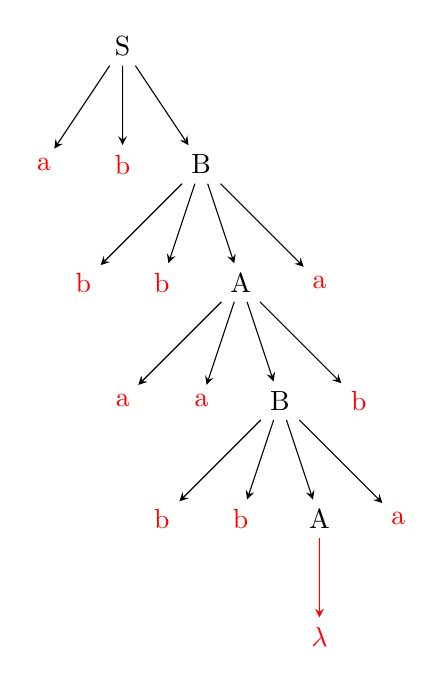
\begin{tikzpicture}
                \node {S} [sibling distance = 1cm]
                        child {node [red]{a} edge from parent} 
                        child {node [red]{b} edge from parent} 
                        child {node {B}
                                child {node [red]{b}}
                                child {node [red]{b}}
                                child {node {A}
                                        child {node [red]{a}}
                                        child {node [red]{a}}
                                        child {node {B}
                                                child {node [red]{b}}
                                                child {node [red]{b}}
                                                child {node {A}
                                                        child [red]{node{$\lambda$}}        
                                                }
                                                child {node [red]{a}}
                                        }
                                        child {node [red]{b}}
                                }
                                child {node[red]{a}}
                        edge from parent}

                ;
        \end{tikzpicture}
\end{figure}


\section*{Problem 9(d)}

\textbf{Find a context free grammar for $\mathbf{ L = \left\{  a^nb^m \; : \; 2n \leq m \leq 3n,\, n \geq 0,\, m \geq 0  \right\} }$}

Consider the grammar $G = \left\{ \{S\}, \{a,b\}, S, P \right\}$, with productions:
\begin{gather*}
        S \rightarrow aSbb \\
        S \rightarrow aSbbb \\
        S \rightarrow \lambda \\
\end{gather*}

If you only ever apply the first rule, you will have twice as many $b$'s as $a$'s.
If you only ever apply the second rule, you will have three times as many $b$'s as $a$'s.

If you mix them up, you cannot go below the lower bound of $2n$, and cannot go above the upper bound of $3n$, so it will be somewhere
between $2n$ and $3n$, so the grammar defines the language.

\section*{Problem 12(b)}
\textbf{Find a context free grammar for \\ $\mathbf{ L = \left\{  a^nb^mc^k \; : \; n = m \text{ or } m \neq k    ,\, n \geq 0,\, m \geq 0 ,\, k \geq 0  \right\} }$}

Consider the grammar $G = \left\{ \{S, E, N, D, A, B^+, C, C^+\}, \{a, b, c\}, S, P \right\}$, with productions:
\begin{align*}
                S \rightarrow EC \, | \, AN & hello \\
                A &\rightarrow aA \, | \, \lambda\\
                B^+ &\rightarrow bB^+ \, | \, b \\
                C &\rightarrow cC \, | \, \lambda \\
                C^+ &\rightarrow cC^+ \,|\, c \\
                E &\rightarrow  a E b \, | \, \lambda\\
                N &\rightarrow B^+D \, | \, DC^+ \\
                D &\rightarrow bDc \, | \, \lambda \\
\end{align*}

This one isn't very concise or elegant, but the idea is that you:
\begin{itemize}
        \item Decide whether you want $n=m$ ($E$) or $m \neq k$ ($N$)
        \item If $E$qual:
        \begin{itemize}
                \item Leave room for as many $c$'s as you want on the end
                \item Nest as many $aEb$'s as you want
        \end{itemize}
        \item If $N$ot equal
        \begin{itemize}
                \item Leave room for as many $a$'s as you want at the front
                \item Choose which letter is going to have more than the other, generate at least one of those
                \item Nest $D$own as many $bDc$'s as you want
        \end{itemize}
\end{itemize}

\end{document}